\chapter{机器人安全验证平台}
强化学习方法在机器人控制任务中表现出良好的决策能力，但其在实际部署过程中仍面临显著的 sim-to-real gap 问题，尤其是在安全约束严格的应用场景中，策略在仿真环境中的有效性难以直接迁移到真实机器人系统。
另一方面，现有强化学习算法通常依赖于高并行度的训练环境以提升样本效率，而主流机器人仿真平台（如 Gazebo 和 Webots）在设计上更侧重于物理仿真与单实例交互，难以直接支持大规模并行训练。
因此，构建一个具备安全性验证能力且易于迁移至真实系统的中间验证平台具有重要意义。

基于上述背景，本文设计并实现了一套支持远程访问的机器人仿真验证平台。该平台通过浏览器端提供统一的实验入口，用户无需在本地部署复杂的机器人软件环境，即可远程访问仿真系统并执行算法验证任务。

% 对于RoboticsAcademy的改进：支持webots、支持多机器人实验、添加编队实验场景

\section{平台层次架构}

为支持安全强化学习算法在机器人系统中的高效验证，本文设计了面向仿真与真实系统统一的分层架构。该架构以模块解耦与接口标准化为核心原则，通过多层协同实现从算法开发到仿真验证再到系统部署的完整流程。平台总体结构如图~\ref{fig:platform_framework}所示，主要包括仿真与硬件层、中间件层、容器化后端层、应用与接口层以及前端交互层。

\textbf{（1）仿真与硬件层}作为系统的基础支撑层，负责构建机器人运行环境并提供物理交互基础。在仿真层面，平台基于 Gazebo 与 Webots 构建高保真机器人仿真环境，用于模拟多种机器人模型及复杂场景；在硬件层面，该结构可无缝扩展至真实机器人系统，从而支持算法的实际部署与验证。

\textbf{（2）中间件层}负责系统各模块之间的数据通信与功能解耦。平台采用 ROS 2 作为核心通信中间件，通过话题发布/订阅机制实现机器人状态信息（如位姿、速度与传感器数据）的实时传输，并支持控制指令的高效下发。同时，ROS 2 的分布式架构为多机器人系统提供了天然支持，使平台能够扩展至多智能体协同任务场景。

\textbf{（3）容器化后端层}用于实现系统运行环境的统一封装与调度管理。平台基于 Docker 构建容器化运行环境，将仿真系统、ROS 2 中间件以及算法模块集成于独立容器中。通过容器化部署，不同实验任务可在隔离环境中独立运行，从而保证实验结果的可复现性，并支持多场景并行执行与动态调度。

\textbf{（4）应用与接口层}是安全强化学习算法的执行核心。该层通过硬件抽象接口（HAL）对底层通信机制进行封装，使算法开发者能够以统一接口获取传感器数据并发送控制指令。同时，该层集成控制执行框架，实现感知、状态估计、策略计算与控制输出的闭环流程，并提供可视化接口以支持算法调试与结果分析。

\textbf{（5）前端交互层}作为系统的用户交互入口，实现远程访问与实验管理功能。用户无需在本地部署复杂环境，即可通过前端界面完成代码编写、仿真控制与运行监控。前端通过 WebSocket 与后端建立实时通信连接，实现机器人状态数据的动态更新与控制指令的低延迟传输。

通过上述分层架构设计，平台实现了机器人系统各功能模块之间的解耦与协同。该架构不仅提升了系统的可扩展性与可维护性，也为安全强化学习算法的系统化验证提供了稳定可靠的实验基础。

\begin{figure}
    \centering
    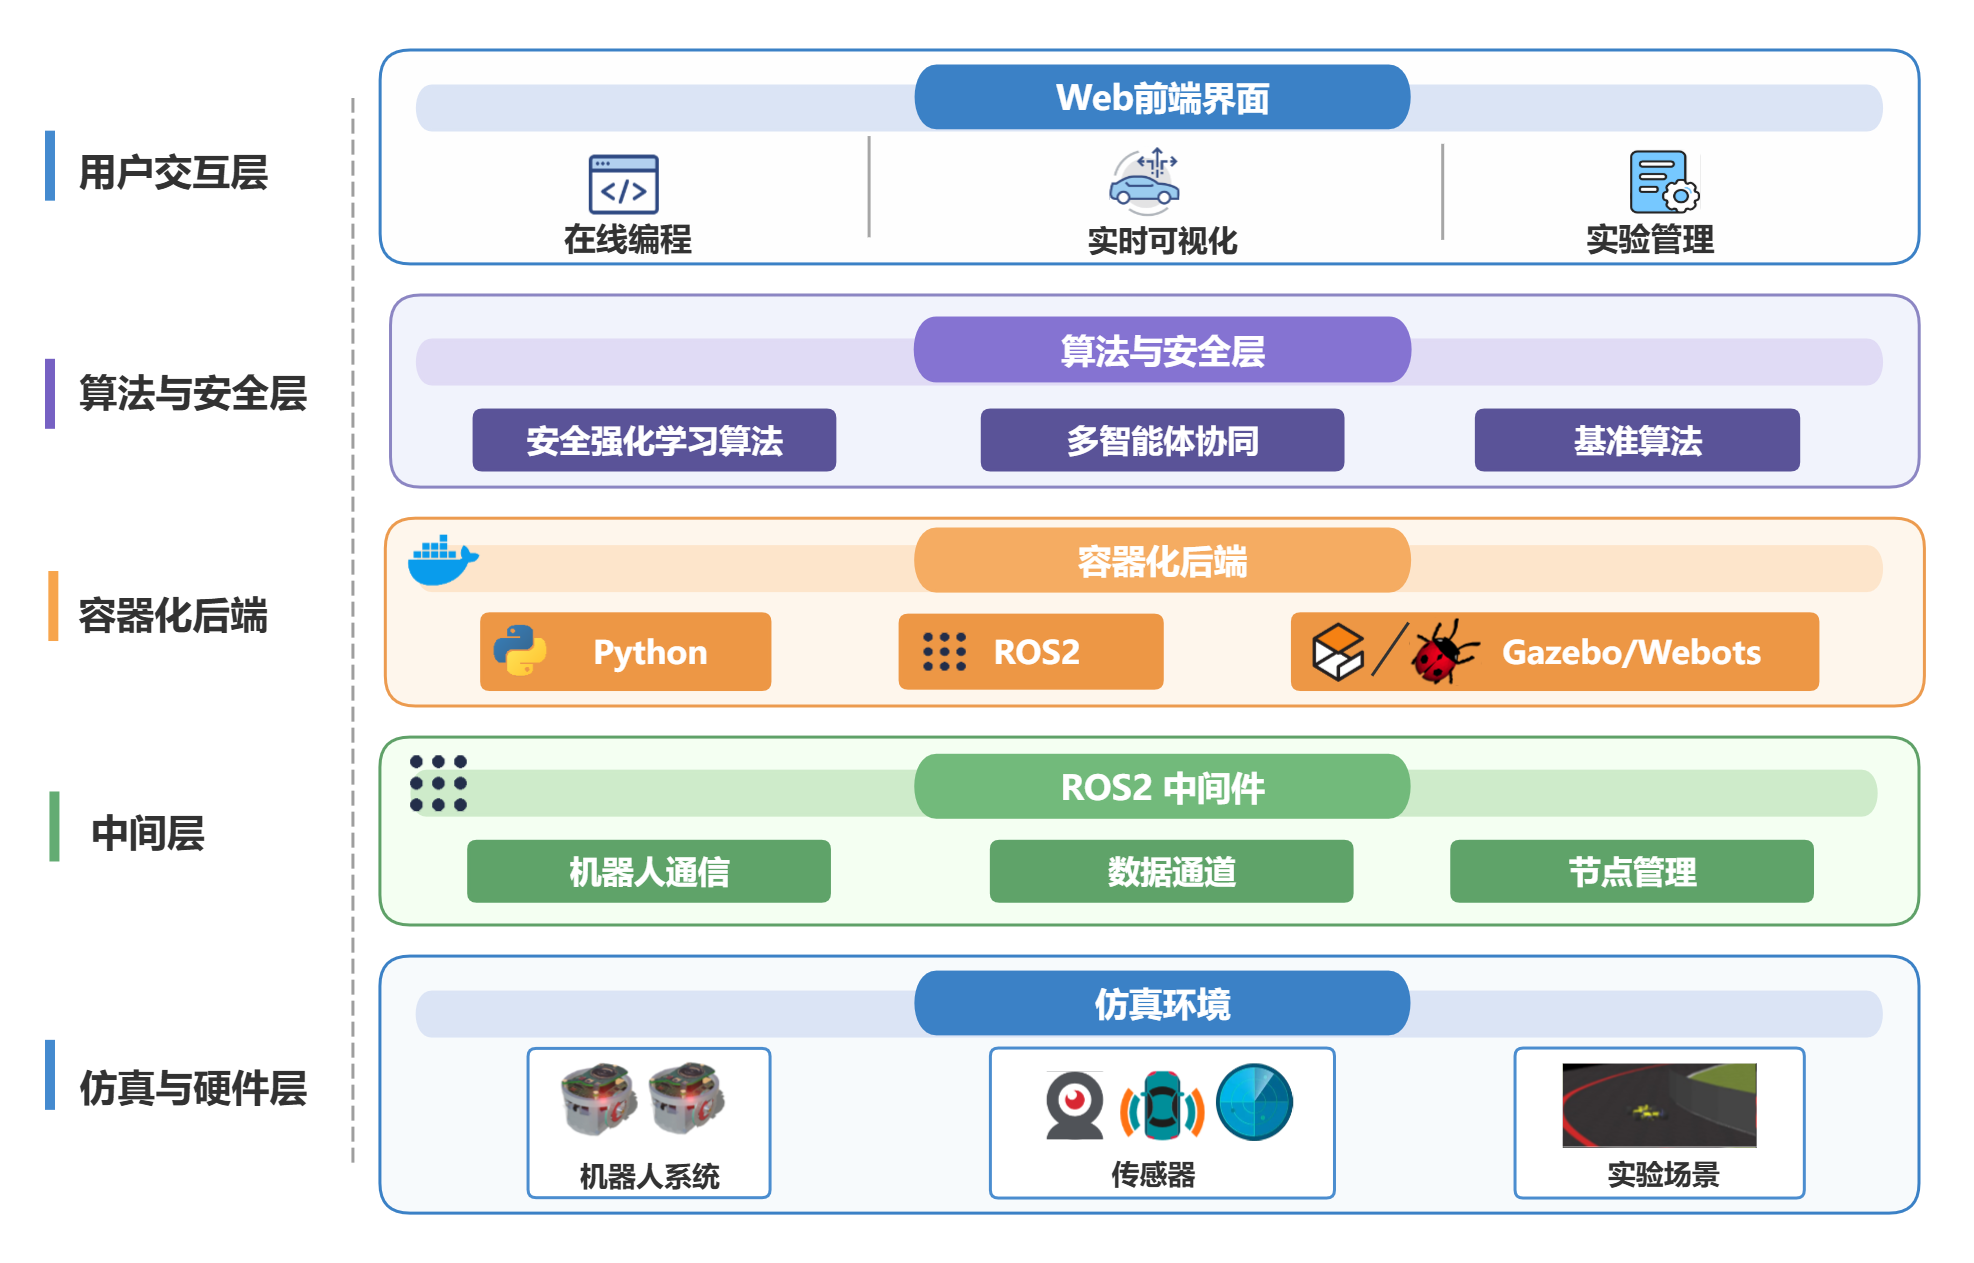
\includegraphics[width=1\linewidth]{images/platform_framework.png}
    \caption{Enter Caption}
    \label{fig:platform_framework}
\end{figure}

\section{核心机制设计}

在上述分层架构基础上，为提升平台在安全强化学习场景下的易用性，本文围绕实验可复现性、系统可解释性以及交互实时性，设计了三项关键机制：容器化并行调度机制、双通道可视化机制以及基于 WebSocket 的实时通信机制，从而提升平台性能与用户体验。

\subsection{容器化与并行调度机制}

针对强化学习算法对高并行训练环境的需求，以及机器人仿真环境在部署与依赖管理方面的复杂性，平台采用基于 Docker 的容器化运行机制对实验环境进行统一封装。

容器化运行机制中，每个实验任务均运行于独立的容器实例中，容器内部集成仿真引擎（如 Gazebo、Webots）、ROS 2 中间件以及算法执行模块。该设计使不同实验之间在软件依赖、运行状态及资源使用上实现完全隔离，从而避免环境冲突问题。同时，容器镜像在构建阶段已固定所有依赖版本，确保实验在不同时间与不同设备上的一致性，从而提升实验结果的可复现性。

在此基础上，平台通过容器调度机制支持多实例并行运行。后端系统根据用户请求动态创建、启动或销毁容器，实现实验任务的按需分配与资源管理。该机制不仅能够支持多用户并发访问，还可为强化学习算法提供并行环境，从而提升样本采集效率与训练速度。

\subsection{双通道可视化机制}

为提升机器人系统运行状态的可解释性与调试效率，平台设计了一种融合语义级状态表达与原生仿真界面展示的双通道可视化机制。

语义级可视化通道（WebGUI）从仿真环境中提取机器人位姿、传感器读数以及安全约束等关键状态信息，并将其统一组织为结构化数据，通过 WebSocket 实时推送至前端。前端采用组件化渲染方式，将上述数据映射为轨迹曲线、激光扫描、力向量以及约束边界等二维或抽象图形，从而直观呈现算法的内部状态与决策过程，使系统运行逻辑具备更强的可分析性与可解释性。

原生界面可视化通道（noVNC）则对仿真软件（如 Gazebo、RViz 或 Webots）的图形界面进行远程转发。后端依托虚拟显示技术启动图形化进程，并通过 VNC 协议将渲染结果实时传输至浏览器端，再以嵌入式页面形式进行呈现，从而完整保留原生仿真工具的交互能力与视觉效果，使用户能够获得与本地运行一致的使用体验。

该可视化机制通过语义层表达与原生图形复现的协同设计，同时支持对算法状态的细粒度分析与对仿真场景的完整观测，从不同维度增强系统整体的可视化表达能力。

\subsection{安全评估验证机制}
针对安全强化学习研究中实验结果难以复现、不同方法之间缺乏统一评估标准的问题，平台设计了一种统一的安全评估与模型验证机制，用于对不同算法在一致条件下进行系统性比较。

该机制首先对实验环境与任务配置进行标准化描述，包括机器人模型、场景结构、障碍物分布以及传感器参数等信息。所有算法均在相同环境配置下运行，从而消除外部因素对实验结果的影响。在此基础上，平台定义统一的评估指标体系，对算法性能进行多维度量化分析。

评估指标不仅包含传统强化学习中的任务完成率与累计奖励，还重点引入与安全相关的度量，例如约束违反次数、最小安全距离以及累计安全代价等。通过对安全性与任务性能的联合评估，可以更加全面地反映算法在复杂环境中的实际表现。

为支持已有模型的复现与对比，平台提供模型导入与验证接口。用户可以上传训练完成的策略模型文件，系统在加载模型后自动执行标准化验证流程，包括环境初始化、策略推理以及结果记录。该机制使不同来源的算法能够在统一平台上进行直接对比，避免因实现差异带来的评估偏差。


\section{系统实现}
为进一步明确系统功能组成与模块职责，本文从功能实现角度将平台划分为机器人仿真模块、前端交互模块、后端服务模块以及机器人通信模块四个核心模块。本节对平台各核心模块的具体实现进行说明。

\subsection{机器人仿真模块}
机器人仿真模块负责构建算法运行环境，并为控制策略提供可控且可复现的实验条件。系统采用 Docker 对仿真环境进行容器化封装，每个实验任务对应独立容器实例。容器内部集成仿真引擎、ROS 2 中间件及算法运行依赖，从而实现运行环境隔离，避免依赖冲突问题。
当用户启动某个实验任务时，系统会自动创建并启动对应的仿真容器，从而完成实验环境的初始化。

系统仿真引擎选用 Gazebo 与 Webots，两者均具备高保真物理建模能力以及丰富的机器人模型与传感器支持。通过配置文件描述实验场景，包括机器人结构、环境地图及障碍物分布，系统可按任务需求动态加载对应仿真环境，保证实验条件一致性。
用户编写的机器人控制程序在仿真环境中运行，获取机器人状态信息，并向机器人执行器发送控制指令，从而实现完整的机器人控制闭环。

ROS 2 节点负责连接仿真环境与算法模块。仿真器通过接口桥接发布机器人状态信息，包括位姿、速度及激光或视觉传感器数据；控制节点订阅相关话题并输出控制指令，形成闭环控制流程。所有话题名称与消息类型通过配置文件统一定义，从而保证不同任务之间接口一致。

图形界面通过虚拟显示机制提供。容器内部启动 Xvfb 或 Xvnc 构建虚拟显示环境，仿真程序在该显示环境中运行。VNC 服务将图像帧编码后通过网络传输至前端浏览器，实现远程渲染。用户可以通过浏览器实时查看机器人在环境中的运动状态，并根据实验结果对控制算法进行调整。

仿真模块周期性输出运行数据，包括机器人状态、传感器信息及控制量，并通过通信模块发送至前端，为状态可视化与算法分析提供数据支持。

本文通过容器化部署与仿真平台集成，构建了一个稳定、可扩展的机器人仿真环境，为机器人算法提供真实感较高的仿真测试场景，并保证实验环境的一致性与可复现性，为多机器人强化学习算法的实验验证提供了可靠的平台支持。

\subsection{前端交互模块}

前端交互模块基于单页应用（SPA）架构实现，采用 React 与 TypeScript 构建组件化界面。系统通过统一状态管理与路由机制组织各功能模块，从而提升整体可维护性与扩展能力。

\subsubsection{任务管理界面}

任务管理界面模块用于展示平台中可用的机器人实验任务，并提供实验任务的选择与管理功能。如图~\ref{fig:tasks}所示，用户可以通过该界面浏览平台中的实验场景列表，并查看每个任务的基本信息，例如任务名称、任务描述以及运行状态。

当用户选择某个实验任务时，前端系统会向后端服务器发送请求，获取对应任务的配置数据，并加载相应的仿真环境和界面组件。
\begin{figure}
    \centering
    
\includegraphics[width=1\linewidth]{images/tasks.png}
    \caption{任务管理界面}
    \label{fig:tasks}
\end{figure}

\subsubsection{任务运行界面}
任务运行界面通过向用户提供在线代码编辑器、任务控制面板以及仿真可视化窗口，使用户能够在浏览器环境中完成机器人算法的编写、运行与调试。如图~\ref{fig:follow_line}所示，页面左侧为代码编辑区，右侧为仿真可视化区及终端调试区，右上方任务控制面板用于管理实验流程与系统运行状态。
\begin{figure}
    \centering
    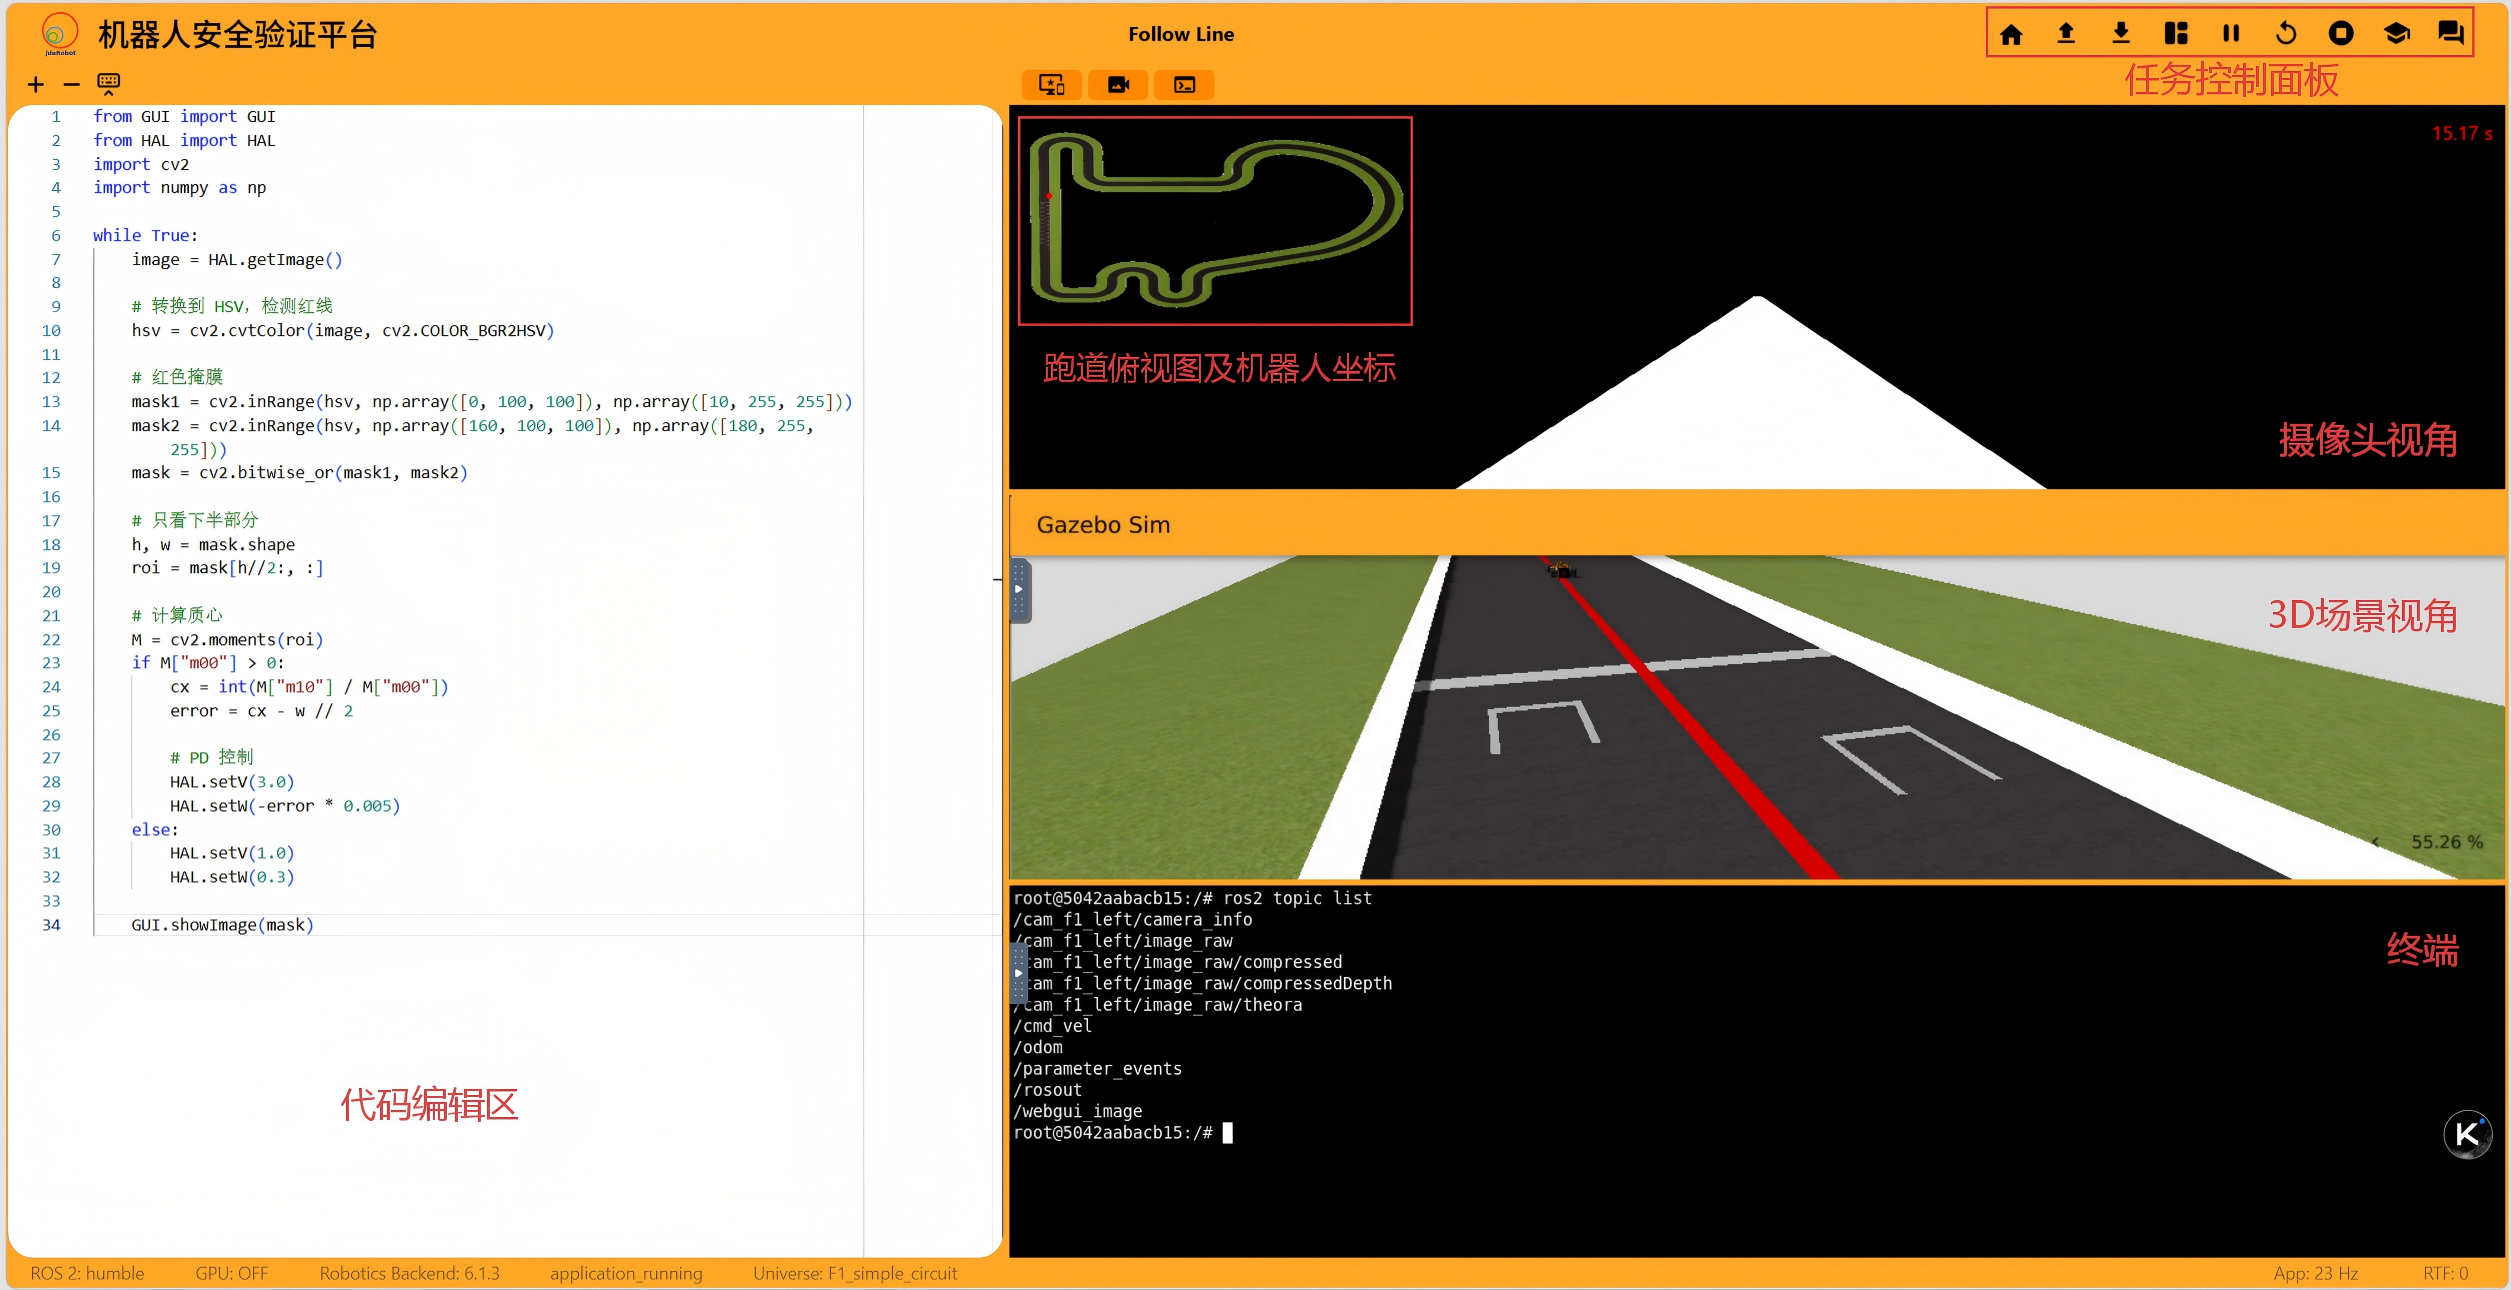
\includegraphics[width=1\linewidth]{images/follow_line(1).png}
    \caption{实验界面}
    \label{fig:follow_line}
\end{figure}

\paragraph{代码编辑区}
代码编辑区通过集成 IDE 组件实现代码编辑功能。
该模块支持在线代码编辑，并提供语法高亮、代码自动补全等功能，提高代码编写效率。同时系统允许用户选择不同的仿真环境或机器人模型配置实验环境。用户通过界面按钮可以启动、暂停或重新运行机器人程序。此外，系统支持代码文件的加载、保存以及模板文件下载。通过上述功能，系统为用户提供了类似本地开发环境的在线编程体验，使机器人算法开发过程更加便捷。

\paragraph{可视化展示区}
可视化展示区主要用于展示机器人仿真环境以及实验运行状态。该模块通过用组件级数据可视化（WebGUI）与桌面级远程可视化（noVNC）并行的方式进行实现。
数据可视化通过接收后端周期性推送的状态数据，并映射为二维图形，从而实现对系统状态的语义化表达。事件驱动触发局部组件更新的机制减少了不必要的重绘，提高了渲染效率。
远程桌面通过 Xvnc 与 noVNC 将图形界面以远程帧缓冲形式传输至浏览器，前端通过 iframe 加载对应页面，实现对 Gazebo、Webots 等原生界面的无侵入式展示。
此外，系统通过状态机驱动可视化组件的加载与显示，并支持多面板动态编排。

\paragraph{终端调试区}
终端调试区提供对后端运行环境的直接访问能力，支持实时查看程序执行过程中的标准输出与错误信息，从而辅助系统状态分析与问题定位。该功能通过远程终端机制进行实现。前端基于 noVNC 将容器内的 xterm 图形终端嵌入浏览器页面，实现终端界面的可视化展示。后端在虚拟显示环境中启动 Xvnc 服务与 xterm 进程，构建完整的终端会话，并通过端口映射建立浏览器与容器之间的访问通道。程序运行过程中产生的日志与输出信息通过伪终端（PTY）写入终端设备，由 xterm 解析并更新显示内容，随后经 VNC 协议传输至前端界面。该机制实现了浏览器端对容器内部终端环境的实时访问，保证了调试过程的连续性与交互性。

\subsection{后端服务模块}

后端服务模块基于 Django 框架构建，负责系统业务逻辑处理与资源管理。系统采用 RESTful 架构设计，通过统一 API 向前端提供数据访问接口，实现前后端解耦。

从功能结构上看，后端系统主要承担实验任务管理、API 服务提供、数据库管理以及系统调度与控制几个方面的功能。

\subsubsection{实验任务管理}
实验任务管理模块维护平台中的任务及其配置数据。每个任务包含机器人模型、仿真场景及算法模板等信息。系统根据任务标识读取配置并返回前端，用于初始化仿真环境。

实验任务管理模块负责维护平台中的机器人实验任务及其相关配置。每个实验任务均包含完整的环境描述信息，包括机器人模型、仿真场景、实验工具以及算法模板等。系统通过统一的数据结构对这些信息进行组织和管理，从而使不同实验任务能够在平台中进行统一调度。

当用户在前端界面选择某个实验任务时，后端系统会根据任务标识从数据库中读取对应的配置信息，并返回给前端系统。随后前端根据任务配置加载对应的仿真环境与界面组件，从而完成实验任务的初始化过程。

\subsubsection{API 服务提供}
为了实现前端系统与后端系统之间的数据交互，平台设计了一组 REST API 接口，用于向前端提供统一的数据访问服务。主要接口包括实验任务列表获取、实验配置加载以及代码模板下载等功能。

在系统运行过程中，前端应用通过 HTTP 请求调用相应的 API 接口。例如，当用户进入实验页面时，前端首先调用获取实验列表接口，从后端服务器加载所有可用实验任务；当用户选择具体任务时，系统再调用实验配置接口获取对应的仿真环境信息。这种基于 REST API 的通信方式能够有效降低系统耦合度，并提高系统的可扩展性。

\subsubsection{数据库管理}

为了实现平台资源的统一管理，系统采用 PostgreSQL 作为后台数据库，用于存储实验任务、仿真环境配置以及机器人模型等核心数据对象。PostgreSQL 具有良好的稳定性与扩展能力，能够支持复杂数据结构的存储与查询，适合用于机器人实验平台的数据管理。
在数据库设计方面，平台主要包含以下几个核心数据对象：
\begin{itemize}
    \item Task：具体的机器人实验任务；
    \item Universe：实验任务对应的仿真环境配置；
    \item World：定义具体的仿真场景；
    \item Robot：机器人模型及其控制接口；
    \item Tool：实验过程中使用的辅助工具组件。
\end{itemize}

通过上述数据结构，平台能够对不同机器人实验任务进行统一管理，并支持多种仿真环境配置。同时，Django 提供的对象关系映射（ORM）机制使得开发人员可以通过 Python 对象直接访问数据库，从而简化数据库操作并提高开发效率。

\subsubsection{系统调度与控制}
系统调度模块负责实验任务的生命周期管理。用户触发实验请求后，后端根据配置启动对应容器，并建立通信连接。同时维护运行状态，包括启动、暂停与终止等操作，保证任务执行过程的有序性与稳定性。

通过上述模块设计，后端服务系统实现了机器人实验任务管理、数据服务以及仿真调度等核心功能，为平台提供了稳定可靠的运行基础。同时，基于 RESTful 架构与模块化设计思想，系统具有良好的可扩展性，可以方便地接入新的机器人实验任务与仿真环境，从而满足多机器人强化学习研究的需求。

\subsection{机器人通信模块}
通信模块承担前端、后端与仿真环境之间的数据交互功能。由于机器人实验过程中需要频繁交换状态信息与控制数据，因此需要一种低延迟、高实时性的通信机制来保证数据传输效率。系统采用 WebSocket 建立持久连接，实现低延迟双向通信。

连接建立阶段，前端在实验启动时向后端发起请求，后端创建独立通信会话并返回连接确认信息。连接建立后，系统进入持续数据交互状态。

数据传输的信息包含仿真环境周期性生成的状态数据（如机器人位姿、传感器信息及系统运行状态），和用户触发的控制指令，包括程序执行控制与动作输入。状态数据由后端转发至前端进行实时更新，控制指令则传递至仿真系统完成执行。系统数据链路图如图~\ref{fig:data}所示。

通信模块同时负责运行状态同步与异常反馈。当仿真环境状态发生变化或出现错误时，相关信息将及时传输至前端，从而保证系统状态一致性并提高调试效率。

该通信机制有效降低了数据传输延迟，提升了系统交互实时性，为机器人在线仿真与安全策略验证提供了稳定的数据通道。
\begin{figure}
    \centering
    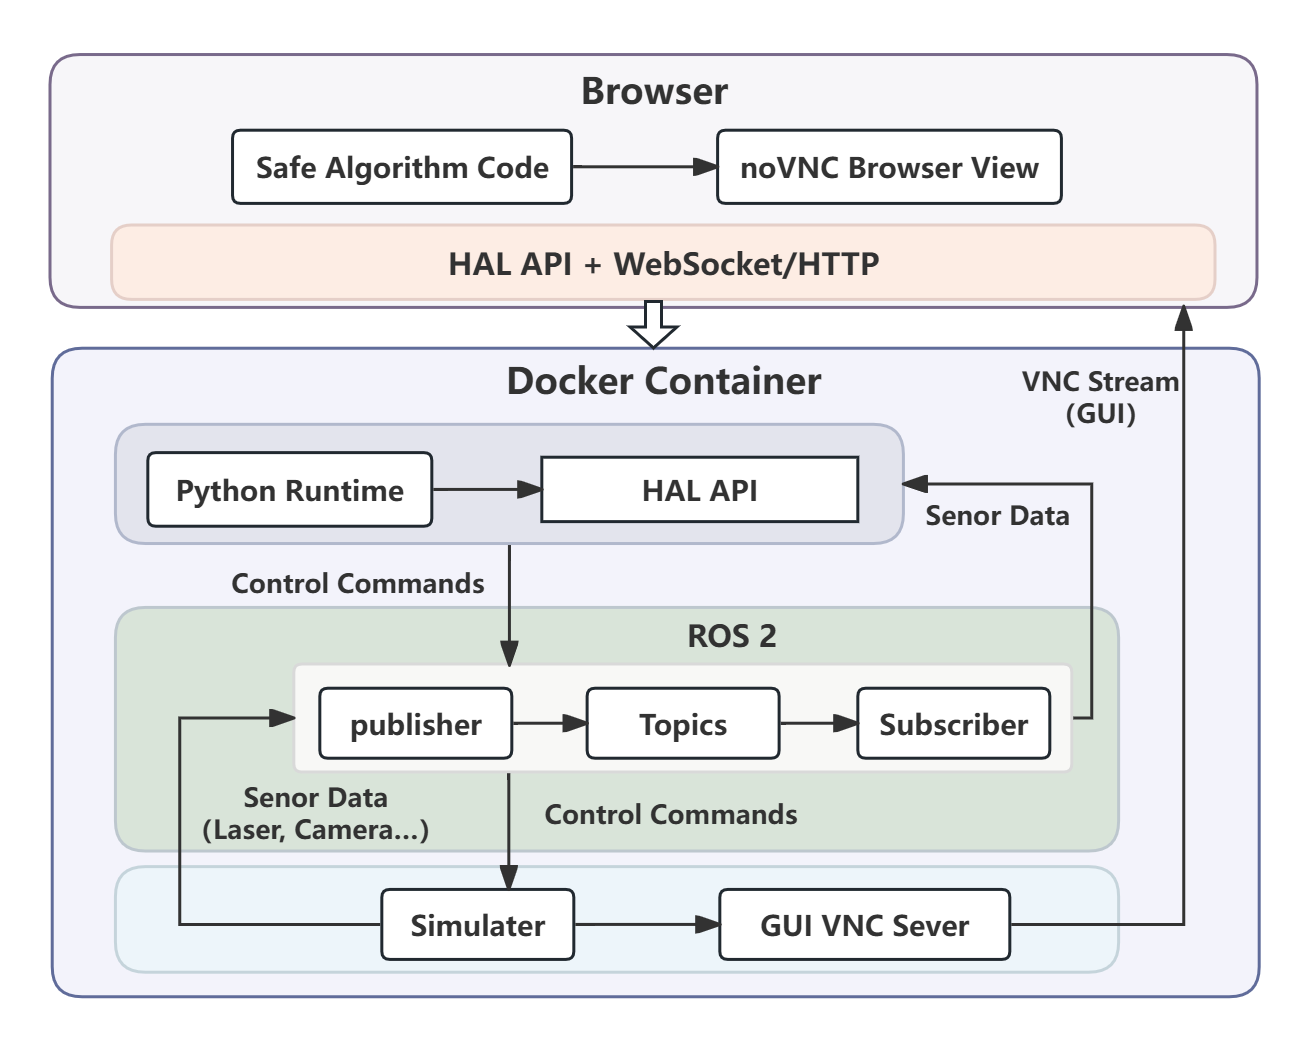
\includegraphics[width=1\linewidth]{images/platform data stream.png}
    \caption{系统数据链路图}
    \label{fig:data}
\end{figure}
\section{本章小结}

本章围绕安全强化学习算法的验证需求，设计并实现了一套面向机器人系统的仿真验证平台。针对传统机器人仿真环境在可复现性、并行能力以及安全验证支持方面的不足，平台从体系结构与关键机制两个层面进行了系统设计。

在体系结构上，平台采用分层架构，将仿真环境、通信中间件、容器化运行环境、算法执行逻辑以及前端交互界面进行解耦，实现了系统功能的模块化组织与统一接口管理。在此基础上，进一步通过容器化技术构建标准化运行环境，使不同实验任务能够在隔离条件下稳定运行，并支持多实例并行调度。

在关键机制方面，平台设计了容器化并行调度机制、双通道可视化机制以及基于 WebSocket 的实时通信机制。其中，容器化机制保证了实验环境的一致性与可复现性；双通道可视化机制实现了机器人运行状态的语义表达与原生仿真展示的有机结合；实时通信机制则为系统提供了低延迟的数据交互能力，确保了仿真过程的实时性与交互性。

在具体实现上，系统完成了仿真模块、前端交互模块、后端服务模块以及通信模块的开发，构建了从任务管理、环境部署到运行监控的完整流程。通过统一的数据接口与调度机制，各模块之间实现了高效协同，能够稳定支持多场景、多任务的机器人算法验证。

本章所构建的机器人安全验证平台为后续安全强化学习算法的实验研究提供了统一、可扩展且具有良好可解释性的基础环境，为多机器人系统在复杂场景下的安全决策研究奠定了支撑。
